\documentclass[]{article}
\usepackage[margin=2.5cm]{geometry}
\usepackage{tikz}
\begin{document}


\textbf{Teorema: Una arista $e$ es una arista de corte sii no pertenece a ningún ciclo} 
\\ 
\\
Sea $W(G)$ la cantidad de componentes de un grafo $G$, decimos que una arista es de corte sii $W(G - e) > W(G)$, es decir que al eliminar la arista el número de componentes sea mayor al del grafo original ($G$). \\ \\

	\begin{center}
	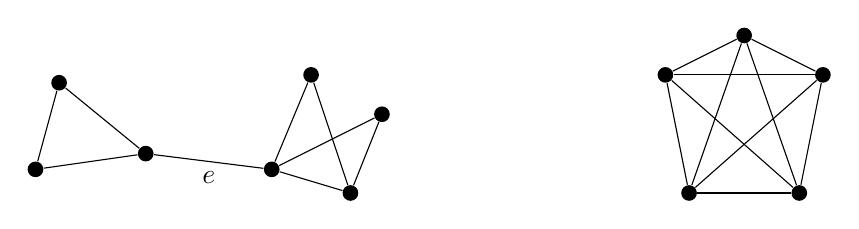
\begin{tikzpicture}
		
	    %Nodos de grafo con aristas de corte
		\node[fill, inner sep=2pt, circle] (A1) at (0,0.3) {};
		\node[fill, inner sep=2pt, circle] (A2) at (1,0) {};
		\node[fill, inner sep=2pt, circle] (A3) at (1.4,1) {};
		\node[fill, inner sep=2pt, circle] (A4) at (0.5,1.5) {};
		\node[fill, inner sep=2pt, circle] (A5) at (-1.6,0.5) {};
		\node[fill, inner sep=2pt, circle] (A6) at (-3,0.3) {};
		\node[fill, inner sep=2pt, circle] (A7) at (-2.7,1.4) {};
		
		% Nodos de Grafo sin aristas de  k5
		\node[fill, inner sep=2pt, circle] (A) at (5, 1.5) {};
		\node[fill, inner sep=2pt, circle] (B) at (5.3, 0) {};
		\node[fill, inner sep=2pt, circle] (C) at (7,1.5) {};
		\node[fill, inner sep=2pt, circle] (D) at (6, 2) {};
		\node[fill, inner sep=2pt, circle] (E) at (6.7,0) {};
		
		% Dibujando aristas del grafo con aristas de corte
		  \draw (A1) -- (A2);
		  \draw (A1) -- (A4);
		  \draw (A1) -- (A3);
		  \draw (A3) -- (A2);
		  \draw (A4) -- (A2);
	     \draw (A1) -- (A5) node[midway, below] {$e$};
		  \draw (A5) -- (A6);
		  \draw (A7) -- (A6);
		  \draw (A7) -- (A5);
		
		% Dibujando aristas de k5
		\foreach \from/\to in {A/B, A/C, A/D, A/E, B/C, B/D, B/E, C/D, C/E, D/E}
		\draw (\from) -- (\to);
		
	\end{tikzpicture}
	
    \hspace{1.3 cm}	$W(G - e)  > W(G )$  \hspace{3cm} Grafo sin aristas de corte 
	
	
\end{center}

Note que para que $e$ sea una arista de corte $\exists \: u,v \in V(G)$ tal que  $u,v$ son adyacentes en $G$. Pero no lo son en $G - e $, es decir todo $uv$-camino contiene  a $e$ (definición arista de corte )
 \\ 
 \\
\textbf{Lema}: Dado $e$ una arista de corte $\exists \: u,v \in V(G) $ tal que $u,v$ son adyacentes en $G$ y $u,v$ NO son adyacentes en $G - e$ sii todo $u,v$-camino contiene a e. 
\\ 
\\
\textbf{Demostración:} $e$ es de corte sii $e$ no pertenece a ningún ciclo.  $ \equiv  \: \: e$ NO es arista de corte sii $e$ pertenece a un ciclo . ($p \iff q  \equiv   \neg p \iff \neg q $ ).
\\
\\ 
Note que si $e$ esto implica que $W(G) = W(G - e)$ de este modo la proposición  anterior es equivalente a demostrar  que:  $W(G) = W(G - e)$ sii $e$ pertenece a un ciclo . ($p \iff q  \equiv   \neg p \iff \neg q $ ).
\\
\\ 
Sin perdida de generalidad suponga que $G$ es conexo, ya que de otro modo usamos la componente conexa a la que $e$ pertenece.
\\
\\
$\Rightarrow$
\\

Luego de aclarar que $G$ es conexo y por hipostesis $G-e$ también lo es, suponga que una arista $e$ que relaciona a $uv$. Por lo tanto $\exists \:\: uv$-trayectoria que vamos a llamar $C$  en $G-e$ .

\begin{center}
	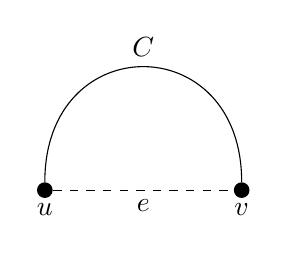
\begin{tikzpicture}
		\node[fill, inner sep=2pt, circle] (u) at (0,0) {};
		\node[fill, inner sep=2pt, circle] (v) at (2.5,0) {};
	    \draw (u) to[out=90, in=90, looseness=2] node[midway, above] {$C$} (v);
		 \draw[dashed] (u) -- (v) node[midway, below] {$e$};
		
		
		\node[below, yshift= -0.05cm] at (u) {$u$};
		\node[below, yshift= -0.05cm] at (v) {$v$};
	
	\end{tikzpicture}
	
	$G - e$
\end{center}
Pero de este modo el camino $Cveu$ es un ciclo en $G$ al que pertenece $e$ (Quedando demostrado en este sentido).
\\
\\	
$\Leftarrow$
\\
\\
Si $e$ pertenece a un ciclo $C = (u, e, v, e_1, v_2, ..., e_k, v_k = u)$ es decir un $u-u$ciclo. Ahora bien en $G-e$, Sean $i,k \in V(G - e)$, del mismo modo $i,k \in V(G)$. Como $G$ es un grafo conexo, observe que $\exists \:\: ik$-camino en $G$ al que llamaremos $C'$ de este modo aparecen dos casos.
\begin{enumerate}
	\item Si $e$ no aparece en $C'$ entonces $C'$ es un $ik$-camino de $G-e$.
	
	\item Si $e$ aparece en $C'$ entonces $C' = (i,b_1,i_2, ..., b_z, u, e, v, b_{j+2}, ...,  k)$.Teniendo en cuenta que $e$ pertenece a un ciclo dada la hipótesis $\exists \:\: C'' = (i, b_1, i_2, ..., u, e_k, v_{k+1},v, b_{j+2}, ...,   k)$. 
	
	
\end{enumerate}

\begin{center}
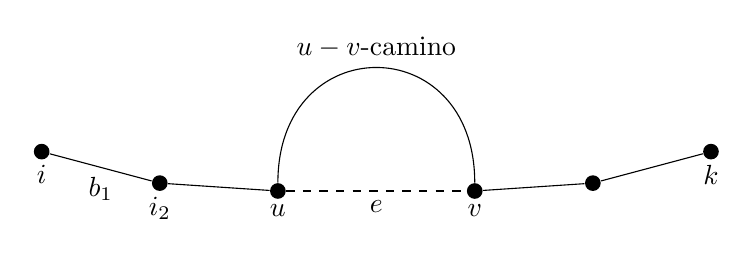
\begin{tikzpicture}
	
	\node[fill, inner sep=2pt, circle] (i) at (-3,0.5) {};
	\node[fill, inner sep=2pt, circle] (i2) at (-1.5,0.1) {};
	\node[fill, inner sep=2pt, circle] (a) at (5.5,0.5) {};
	\node[fill, inner sep=2pt, circle] (k) at (4,0.1) {};
	
	
	\node[fill, inner sep=2pt, circle] (u) at (0,0) {};
	\node[fill, inner sep=2pt, circle] (v) at (2.5,0) {};
	\draw (u) to[out=90, in=90, looseness=2] node[midway, above] {$u-v$-camino} (v);
	\draw[dashed] (u) -- (v) node[midway, below] {$e$};
	\draw (i) -- (i2) node[midway, below] {$b_1$};
	\draw (i2) -- (u);	
	\draw (v) -- (k);
	\draw (a) -- (k);
	
	
	\node[below, yshift= -0.05cm] at (u) {$u$};
	\node[below, yshift= -0.05cm] at (v) {$v$};
	\node[below, yshift= -0.05cm] at (i) {$i$};
	\node[below, yshift= -0.05cm] at (i2) {$i_2$};
	\node[below, yshift= -0.05cm] at (a) {$k$};
	
	
	
\end{tikzpicture}

\end{center}
	


De este modo $C''$ es $ik$-camino en $G-e$, quedando así demostrado que  $G-e$ conexo.


\end{document}
